\documentclass[a4paper,12pt,oneside]{book}
\usepackage{graphicx}
\usepackage[utf8]{inputenc}
\usepackage[T1]{fontenc}
\usepackage{float}
\usepackage[italian]{babel}
\usepackage{listings}
%\usepackage{natbib}
\usepackage{physics}
\usepackage[a4paper, top=2cm, bottom=3cm, right=3cm, left=4cm]{geometry}
\usepackage{amsmath}
\usepackage{bm}
\usepackage{amssymb}
%\usepackage{enumitem}
\usepackage{hyperref}
%\usepackage{booktabs}
\usepackage{subfig}
\usepackage{blindtext}
\usepackage{fancyhdr}
\usepackage{caption}
\usepackage{verbatim}
\usepackage{biblatex}
\addbibresource{bibliografia.bib}

\pagestyle{fancy}

%\title{

%    \begin{figure}[H]
%        \centering
%    
\includegraphics[scale = 0.5 , angle=0]{unipd_logo.png}
%    \end{figure}

%{La formazione delle caustiche nella struttura su grande scala dell'Universo}\\
%\large{Università degli studi di Padova}
%}
%\author{Laureando: Alessandro Bianchetti}
%\date{Anno accademico 2019/20}

\begin{document}

    \begin{titlepage}
    \begin{center}

        \begin{figure}[H]
            \centering
            
\includegraphics[width=0.4\textwidth]{unipd_logo.png}
        \end{figure}

        \vspace{0.5cm}

        \large
        \textbf{UNIVERSITA DEGLI STUDI DI PADOVA}\\
        Dipartimento di Fisica e Astronomia “Galileo Galilei”\\
        Corso di Laurea in Fisica\\

        \vspace{1cm}

        Tesi di Laurea
        \vspace*{1.5cm}

        \LARGE
        \textbf{La formazione delle caustiche nella struttura su grande scala dell'Universo}
        \vspace{1.5cm}

    \end{center}
    \vspace{6cm}
    \small
    \textbf{Relatore: Sabino Matarrese} \\
    \textbf{Laureando: Alessandro Bianchetti}
    \vspace{2cm}

    \LARGE
    \begin{center}
        Anno Accademico 2019/2020
    \end{center}

    

    
\end{titlepage}
	    
    \chapter*{Abstract}
    \blindtext


    \tableofcontents

    \chapter*{Introduzione}
    La presente distribuzione della materia risulta essere altamente disomogenea: si definiscono 
\textit{strutture cosmiche} i colossali ammassi (\textit{cluster}) di galassie tenuti insieme dalla
interazione gravitazionale tra i propri componenti, che raggiungono masse complessive tra $10^{13}$
e $10^{16}$ masse solari. Inoltre esistono sovrastrutture ancora più mastodontiche, dette superammassi.
I superammassi si presentano come un intricato reticolo di filamenti luminosi di galassie, che delimitano
spazi scuri, vuoti. Il fenomeno è noto come \textit{caustiche} e non ha solo applicazione in cosmologia, ma 
risulta trasversale in molteplici situazioni naturali. Il nome caustica si riferisce anche alla scomposizione
della luce sul fondo di una piscina, che ricorda in effetti le distribuzioni galattiche.

\begin{center}
	\begin{figure}[H]
		\centering
		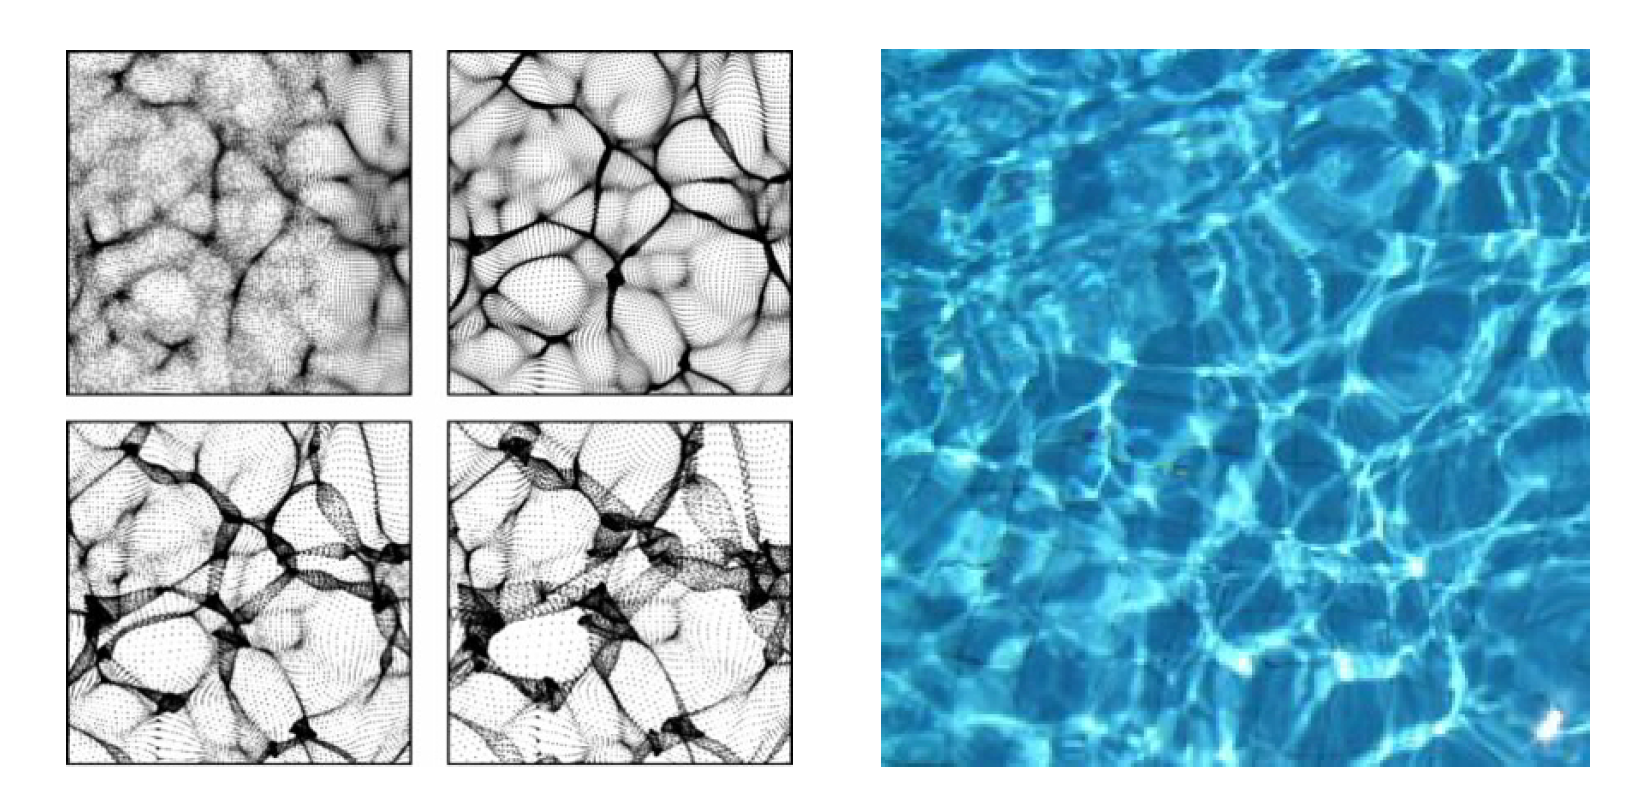
\includegraphics[scale=0.3, angle=0]{caustica.png}
        \caption{A sinistra, simulazione a N corpi bidimensionale fatta in approssimazione di Zel'dovich per crescenti
        oscillazioni di densità rispetto alla media $\rho_b$. A destra, caustica sul fondo di un piscina. Immagine tratta da \cite{gurbatov}.}
		\label{fig:caustica}
	\end{figure}
\end{center}

Questa distribuzione grumosa della massa si può descrivere con preciso approccio matematico, discusso nel primo capitolo,
e riguarda la teoria del \textit{trasporto ottimo}, che affronta proprio il problema di determinare il processo massimamente
efficiente, ovvero con il minimo dispendio, attraverso cui si può trasportare una certa distribuzione di massa iniziale a una 
finale.



    \chapter{Il problema di ricostruzione}
    \begin{comment}
    alcune idee/frasi da inserire:

    Le singolarità sono una caratteristica essenziale di molte discipline, e hanno talvolta conseguenze
    drammatiche sul modello matematico\dots

    Per la risoluzione assumiamo un universo unidimensionale: questa assunzione
    si può giustificare sulla base del fatto che in effetti anche in tre dimensioni i fenomeni di shell-crossing hanno 
    origine unidimensionale con la formazione dei pancakes-
    
    Tuttavia l'analisi offerta sarà facilmente estendibile a più dimensioni.
    
\end{comment}



\section{Equazioni della fluidodinamica}


Una delle ipotesi vertice della seguente trattazione è quella che il plasma primordiale fosse altamente omogeneo.
Tale teoria è avallata dallo spettro della CMB (Cosmic Microwave Background), che risulta riprodurre la stessa
isotropia, eccezion fatta per deboli fluttuazioni termiche che caratterizzavano lo stesso plasma primordiale.

\begin{center}
	\begin{figure}[H]
		\centering
		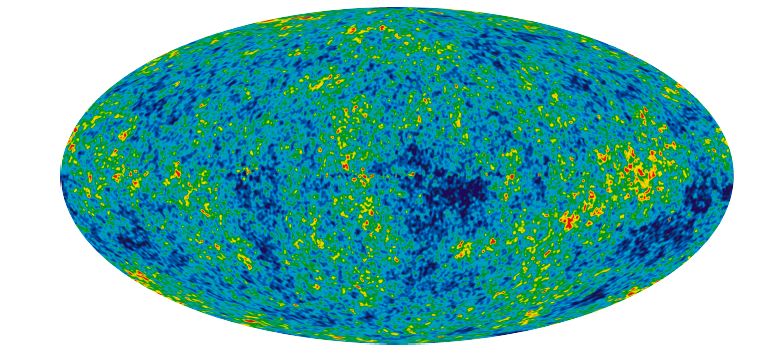
\includegraphics[scale=0.5, angle=0]{cmb.png}
		\caption{Immagine dello spettro della CMB attraverso le misurazioni della sonda spaziale WMAP}
		\label{fig:cmb}
	\end{figure}
\end{center}

Ci muoviamo innanzitutto dal modello cosmologico Einstein-De Sitter, che pone la curvatura dell'universo
e la costante cosmologica $\Lambda$ pari a 0 e prevede uno spazio composto sostanzialmente di materia
oscura fredda (CDM).
In tale cornice definiamo una mappa Lagrangiana $\mathbb{M}: \bm{q} \mapsto \bm{x}(\bm{q}, \tau)$ che connette la posizione
iniziale alla posizione corrente x al tempo di scala $\tau$ $\propto$ $t^{\frac{2}{3}}$.
Inoltre le coordinate x sono coordinate comoventi legate alle coordinate fisiche r dalla relazione
x = r/$a$, dove $a$ rappresenta il fattore cosmico di scala, che corrisponde a $\tau$ in un universo
EdS.
Definiamo infine le velocità $\bm{v} = a \dot{\bm{x}}$ e $\bm{w} = \dot{\bm{r}} = H \bm{r} + v$

Per approcciare la dinamica di particelle non collidenti ("polvere"), definiamo una funzione $f(\bm{x}, \bm{p}, t)$ 
che corrisponde alla densità degli stati nello spazio delle fasi. E' possibile quindi utilizzare il Teorema di 
Liouville, che afferma che la densità sopra citata si conserva nell'evoluzione di un sistema conservativo: in
effetti l'ipotesi di assenza di collisioni ci permette di soddisfare ai requisiti del teorema, e quindi 
possiamo porre a zero la derivata totale della funzione densità, ricavando l'equazione di Vlasov.

\begin{equation}
    \label{eqn:vlasov}
    \frac{\partial f}{\partial t} + \dot{\bm{x}} \nabla_{\bm{x}}f + \dot{\bm{p}} \nabla_{\bm{p}}f  = 0
\end{equation}

L'equazione di Vlasov è molto difficile da risolvere analiticamente: adottiamo quindi un approccio 
teorico semplificato, cioè la descizione Newtoniana di fluido: in particolare sposiamo l'ipotesi 
di entropia costante e di assenza di termini di pressione dal momento che trattiamo la CDM come 
una polvere autogravitante e non collidente.

Il set di equazioni adatto all'approccio fluidodinamico è dato da

\begin{equation}
    \label{eqn:continuità}
    \frac{\partial\rho}{\partial t}\biggr|_{\bm{r}} + \nabla_{\bm{r}}(\rho \bm{w}) = 0
\end{equation}

\begin{equation}
    \label{eqn:eulero}
    \frac{\partial\bm{w}}{\partial t}\biggr|_{\bm{r}} + (\bm{w}\cdot\nabla_{\bm{r}})\bm{w} = - \nabla_{\bm{r}} \Phi
\end{equation}

\begin{equation}
    \label{eqn:poisson}
    \laplacian_{\bm{r}}\Phi = 4\pi G \rho
\end{equation}
dove la (\ref{eqn:continuità}) è l'equazione di continuità che costituisce la conservazione
della massa, la (\ref{eqn:eulero}) è l'equazione di Eulero e viene dalla conservazione del
momento, mentre la (\ref{eqn:poisson}) rappresenta l'equazione di Poisson relativa
al potenziale gravitazionale $\Phi$.

Poniamo inoltre $\rho = \rho_b + \delta\rho$, dove $\rho_b$ è la densità media di background
e $\delta\rho$ costituisce una deviazione da tale valore medio. $\Phi = \Phi_b + \phi{'}$ invece
è la somma di un potenziale di background e un potenziale peculiare $\phi{'}$. Grazie a queste due 
apposizioni possiamo separare l'equazione di Poisson, ottenendo un equazione nella sola coordinata
comovente x.
Possiamo riscrivere anche (\ref{eqn:eulero}) e (\ref{eqn:poisson}) nelle coordinate x, usando la
relazione

\begin{equation}
    \frac{\partial}{\partial t}\biggr|_{\bm{x}} = \frac{\partial}{\partial t}\biggr|_{\bm{r}} + H(\bm{r} \cdot \nabla_{\bm{r}})
\end{equation}

Si ricava dunque

\begin{equation}
    \label{eqn:continuitax}
    \frac{\partial\rho}{\partial t} + 3H\rho +\frac{1}{2}\nabla_{\bm{x}}(\rho\bm{v}) = 0
\end{equation}

\begin{equation}
    \label{eqn:eulerox}
    \frac{\partial \bm{v}}{\partial t} + H \bm{v} + \frac{1}{a}(\bm{v}\cdot\nabla_{\bm{x}})\bm{v} = -\frac{1}{a}\nabla_{\bm{x}}\phi = 0
\end{equation}

\begin{equation}
    \label{eqn:poissonx}
    \laplacian_{\bm{x}}\phi{'} = 4\pi G \delta\rho
\end{equation}

Le equazioni della fluidodinamica rappresentano in effetti uno sviluppo dell'equazione 
di Vlasov fino al primo ordine. Per spiegare questo passaggio, osserviamo che la densità
di massa e la velocità sono associate rispettivamente al momento di aspettazione di ordine 
zero e di primo ordine della densità nello spazio delle fasi $f(\bm{x}, \bm{p}, t)$.

\begin{equation}
    \label{eqn:rho}
    \rho(\bm{x}, t) = \frac{m}{a^3}\int d^3p f(\bm{x}, \bm{p}, t)
\end{equation}

\begin{equation}
    \label{eqn:vel}
    \bm{v}(\bm{x}, t) = \frac{m}{a^3}\frac{\int d^3p \bm{p}f(\bm{x}, \bm{p}, t)}{\int d^3p f(\bm{x}, \bm{p}, t)}
\end{equation}
Integrando ora l'equazione di Vlasov sul dominio del momento $\bm{p}$, si trova che l'ultimo termine
dell'integrando rappresenta un'integrale di volume della forza $\partial f$/$\partial p$, che tramite
il Teorema di Gauss si può riscrivere come un integrale su una superficie all'infinito, dove la forza
si annulla. Utilizzando poi le definizioni (\ref{eqn:rho}) e (\ref{eqn:vel}) si ricava 
\begin{equation}
    \frac{\partial}{\partial t}(a^3 \rho) + \frac{1}{a^2}\nabla_x \int d^3 p \bm{p} f = 0
\end{equation}
maneggiando opportunamente quest'ultima e utilizzando le definzioni fornite in (\ref{eqn:rho}) e (\ref{eqn:vel})
si arriva esattamente all'equazione di continuità (\ref{eqn:continuità}).

Se invece si moltiplica l'equazione di Vlasov per $\bm{p}$ per poi integrare di nuovo su tale variabile, 
conviene lavorare sul termine i-esimo e operare un'integrazione per parti sempre sull'ultimo addendo dell'
integrando.

\begin{equation}
    \frac{\partial }{\partial t} \int d^3 p p^i f + \frac{1}{ma^2} \partial^i \int d^3 p p_j p_j f + a^3 \rho \partial^i \phi = 0 
\end{equation}

Manipolando questa espressione e utilizzando l'equazione di continuità, si arriva proprio all'equazione di Eulero
(\ref{eqn:eulero}.

Le equazioni della fluidodinamica rappresentano dunque i primi termini dello sviluppo dell'equazione di Vlasov,
e perciò costituiscono una via più facilmente percorribile, offrendo la possibilità di giungere a delle soluzioni
analitiche altrimenti proibitive.


\section{Approssimazione di Zel'dovich}

A questo punto tuttavia conviene operare un ulteriore cambio di variabili sul set di equazioni ottenute (\ref{eqn:continuitax}),
(\ref{eqn:eulerox}) e (\ref{eqn:poissonx}). Per farlo si definisce meglio il fattore di scala per mezzo di un'ampiezza $a_{*}$ e
un tempo caratteristico $t_{*}$, in modo che $a(t) = a^{*}(t / t_{*})^{2/3}$. Ricordando inoltre $\rho = \rho_b + \delta\rho$ e 
$\bm{v} = a \dot{\bm{x}}$, facciamo le seguenti sostituzioni

\begin{gather}
    \rho \mapsto \eta = \frac{\rho}{\rho_b} = 1 + \delta \\
    \bm{v} \mapsto \bm{u} = \frac{d\bm{x}}{da} = \frac{d\bm{x}}{dt}\frac{dt}{da} = \frac{\bm{v}}{a\dot{a}} \\
    \phi{'} \mapsto \phi = \frac{3t_{*}^2}{2a_{*}^3}\phi{'}
\end{gather}
Grazie alla mappatura $(\rho, \bm{v}, \phi{'})\mapsto(\eta, \bm{u}, \phi)$, le equazioni del fluido assumono
la nuova forma 

\begin{gather}
    \label{eqn:cont_tau}
    \frac{D\bm{u}}{Da} + \frac{3}{2a}\bm{u} = -\frac{3}{2a}\nabla\phi \\
    \frac{D\eta}{Da} + \eta \nabla \cdot \bm{u} = 0 \\
    \label{eqn:poisson_tau}
    \laplacian \phi = \frac{\delta}{a}
\end{gather}
dove la derivata $D/Da$ si dice \textit{derivata convettiva}.
Ora usiamo il fatto che in un universo EdS linearizzato, la soluzione \textit{growing mode} è data complessivamente
da  $\delta \propto t^{\frac{2}{3}}$, $\bm{v} \propto t^{\frac{1}{3}}$ e $\phi = const$. Con questi andamenti, è
evidente che la nuova coordinata di velocità $\bm{u} = \bm{v} / (a\dot{a}) \approx const$, dal momento che sia 
$\bm{v}$ che $a\dot{a} \propto t^{2/3} \cdot t^{-1/3}$ hanno lo stesso andamento $t^{1/3}$.

Ma allora il termine $Du/Da$ nell'equazione di Eulero si può considerare nullo
\begin{equation}
    \label{eqn:zel}
    \frac{Du}{Da} = 0
\end{equation}
ottenendo così

\begin{equation}
    \label{eqn:zelsol}
    \bm{u} = -\nabla\phi
\end{equation}
che è la soluzione linearizzata, valida per piccole deviazioni dalla densità di background, ovvero per $\delta < 1$.
L'approssimazione di Zel'dovich sta nel considerare tale risultato legittimo anche oltre il regime di linearità, ossia 
assumere la validità di (\ref{eqn:zel}) ovunque.
Si può inoltre osservare che in queste condizioni l'equazione di Poisson gravitazionale risulta disaccoppiata dalle
altre due ed è utile per applicare le condizioni iniziali.
La (\ref{eqn:zel}) descrive un moto rettilineo uniforme, in cui la particella è soggetta solamente alla propria inerzia
senza perturbazioni gravitazionali esterne. Quindi se la posizione iniziale è descritta dalla coordinata lagrangiana
$\bm{q}$, allora per ogni posizione euleriana $\bm{x}$ del moto varrà che 

\begin{equation}
    \bm{u}(\bm{x}, a) = \bm{u}_0(\bm{q})
\end{equation}
Le traiettorie delle particelle, rettilinee e a velocità costante $u$, sono descritte da

\begin{equation}
    \bm{x}(\bm{q, a}) = \bm{q} + a u_0(\bm{q})
\end{equation}
Ma usando (\ref{eqn:zelsol}) si ricaverà

\begin{equation}
    \label{eqn:zelmap}
    \bm{x}(\bm{q, a}) = \bm{q} - a \nabla\phi_0
\end{equation}

Alla fine di questi passaggi si è in grado di identificare la mappa $\mathbb{M}$ che collega le coordinate lagrangiane 
iniziali con quelle finali euleriane. 

A questo punto saremmo in grado di risolvere l'equazione di continuità semplicemente come un'equazione a variabili
separabili, trovando quindi la forma di $\eta$. Tuttavia la via più semplice risulta invece dall'impostare la 
conservazione della massa dei singoli elementi fluidi.

\begin{equation}
    \eta(\bm{x}, a)d^3x=\eta_0(\bm{q})d^3q
\end{equation}
da cui

\begin{equation}
    \eta(\bm{x}(\bm{q}, a), a) = (1 + \delta_0(\bm{q}))\det\left(\frac{\partial q}{\partial x}\right) 
\end{equation}
Ma supponendo che nella configurazione iniizale la perturbazione di energia sia nulla $\delta_0 = 0$
e contemporaneamente utilizzando le proprietà del determinante, si potrà scrivere anche

\begin{equation}
    \eta(\bm{x}(\bm{q}, a), a) = \left[\det\left(\frac{\partial x}{\partial q}\right)\right]^{-1}
\end{equation}
E' possibile scrivere la matrice $\partial x$/$\partial q$ in componenti, sapendo che $x_i = q_i - a \frac{\partial\phi_0}{\partial q^i}$, 
e derivando ulteriormente 

\begin{equation}
    \frac{\partial x^i}{\partial q^j} = \delta^i_j - a \frac{\partial^2 \phi_0}{\partial q_i \partial q^j} = 
    \delta^i_j - a D^i_j(q)
\end{equation}
dove si è definito il tensore di deformazione $D^i_j$, connesso al laplaciano del potenziale gravitazionale. 
Nel sistema di riferimento opportuno tale tensore ha forma
diagonale, con i tre autovalori $\lambda_1(\bm{q})$, $\lambda_2(\bm{q})$ e $\lambda_3(\bm{q})$, dipendenti dalle
coordinate iniziali. Questi governano la deformazione locale della materia lungo i tre assi ortogonali identificati
dagli autovettori. Si può dimostrare che nell'ipotesi in cui il potenziale $\phi_0$ sia gaussiano come previsto
dal meccanismo di inflazione, allora nel almeno uno dei tre autovalori del tensore di deformazione è positivo 
nel 92$\%$ dei casi.
Ora, riscrivendo il rapporto di densità $\eta$

\begin{multline}
    \eta(\bm{x}(\bm{q}, a), a) = \left[\det\left(\frac{\partial x}{\partial q}\right)\right]^{-1} = \left[\det\left( \mathbb{I}- a D \right)\right]^{-1} = \\
    = \frac{1}{(1-a\lambda_1(\bm{q}))(1-a\lambda_2(\bm{q}))(1-a\lambda_3(\bm{q}))}
\end{multline}

A questo punto, è evidente che, supponendo che $\lambda_1(\bm{q})$ sia l'autovalore maggiore, allora il tempo 
$\bar{a}=1/\lambda_1(\bm{q})$ rappresenta la prima criticità, in quanto la quantità $\eta$ diverge e con essa la 
densità. Questo tipo di evento è detto \textit{shell-crossing} o \textit{caustica} ed è rappresenta il 
fenomeno che si registra quando due particelle con diverse coordinate lagrangiane iniziali 
$\bm{q}_1$ e $\bm{q}_2$ confluiscono nella stessa coordinata di campo $\bm{x}$, dando luogo a densità
infinita. 
Tale divergenza è racchiusa nella mancata biunivocità della mappa $\mathbb{M}^{-1}$, dal momento che a 
una sola coordinata euleriana possono corrispondere più coordinate iniziali. A causa della mancanza
di tale biunivocità, la matrice Jacobiana $\partial x/\partial q$ risulta essere mal definita.
Le caustiche delimitano le zone del cosiddetto \textit{multistreaming}, regioni entro le quali non è
più possibile ritracciare le particelle all'indietro, in quanto non sappiamo come si sono comportate
negli eventi di shell-crossing. Le strutture di materia che si formano sono detti \textit{pancakes},
strutture oblate che si sviluppano su un piano, nel senso che la grumosità si sviluppa 
sostanzialmente in una oppure due direzioni. Queste strutture saranno l'opportuna sede la formazione
delle galassie.

Nel regime di single-stream l'approssimazione di Zel'dovich è opportuna, in quanto costitusice 
un modello non accelerato dove le particelle procedono imperturbate lungo una traiettoria rettilinea
 e a velocità costante. Tuttavia a partire dal primo shell-crossing l'approssimazione perde di validità, 
in quanto non prevede effetti di accelerazione gravitazionale esercitata dalle particelle vicine, che 
modificherebbe il cammino della particella in modo sensibile. 

\section{Metodi di ricostruzione}

Come anticipato all'inizio del capitolo, l'alta uniformità della CMB è una prova forte dell'omogeneità 
dell'Universo primordiale. La grumosità della distrubuzione attuale della massa si spiega invece con 
la formazione di strutture filiformi e oblate come i pancakes. Per poter rendere conto di questa transizione,
sono possibili due tipi di atteggiamento: un \textit{forward approach}, che si basa sull'ipotizzare un 
modello iniziale, presumibilmente a densità costante, ed eseguire una simulazione a N corpi sulle basi 
della dinamica Newtoniana, e controllare il grado d'accordo tra l'output della simulazione e la 
distrubuzione attuale delle galassie, per poi accettare o eventualmente rigettare il modello iniziale.
Tale approccio è praticabile solo tramite tecniche numeriche e non permette di formulare analiticamente
il problema a causa del numero troppo elevato di gradi di libertà.

Un modo di ottenere soluzione analitiche invece è seguire un approccio di \textit{reconstruction}, in cui
si tenta di fittare in modo esatto la distribuzione di massa attuale dell'universo e di mappare la velocità 
delle galassie, per poi invertire il problema usando le posizioni attuali come posizioni iniziali e 
cambiando segno alla velocità. 
Tuttavia mentre l'approccio forward, pur con il suo alto coefficiente di difficoltà, si può formulare
in un ben definito problema di Cauchy che garantisca l'unicità delle soluzioni, la reconstruction non
si può formulare allo stesso modo, dato che si è osservato che a causa dello shell-crossing a una 
coordinata euleriana possono corrispondere più posizioni iniziali. Quindi con la ricostruzione si pone 
un problema di condizioni al contorno, per cui la sfida consiste nel trovare un algoritmo che garantisca
unicità.

\begin{center}
	\begin{figure}[H]
		\centering
		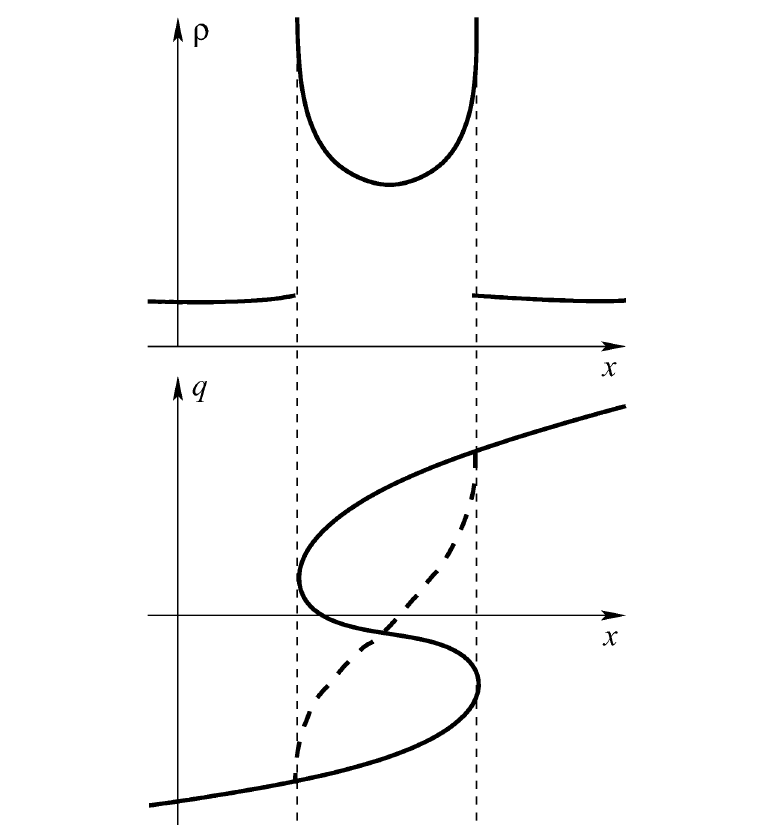
\includegraphics[scale=0.5, angle=0]{rec.png}
        \caption{Esempio di ricostruzione senza unicità. La densità nel grafico superiore potrebbe essere stata generata
        sia dalla mappa lagrangiana in grassetto che da quella tratteggiata. FIgura tratta da \cite{matarrese}}
		\label{fig:rec}
	\end{figure}
\end{center}


Una via percorribile è rappresentata dal problema variazionale come fu formulato da Peebels in \cite{peebles}.
Anzichè risolvere le equazioni del moto, è possibile cercare i punti stazionari della corrispondente
azione di Eulero-Lagrange, scritta nelle coordinate comoventi $\bm{x}$ come

\begin{equation}
    \label{eqn:azione}
    S = \int_0^{t_0} dt \left[\frac{m_i a^2 \dot{\bm{x}}_i^2}{2} - \frac{Gm_i m_j}{a|\bm{x}_i-\bm{x}_j|}+\frac{2}{3}\pi G\rho_ba^2 m_i \bm{x}_i^2\right]
\end{equation}
dove $t_0$ rappresenta il tempo attuale, $\bm{x}_i$ è la traiettoria della i-esima particella e $\rho_b$
è la densità media di background. Se denotiamo come $\mathcal{L}$ l'integrando di (\ref{eqn:azione}), allora
è possibile calcolare la variazione di azione e porla uguale a zero per cercare le orbite stazionarie.

\begin{equation}
    \delta S = \int_0^{t_0} dt \left[\frac{\partial \mathcal{L}}{\partial \bm{x}_i}\cdot \delta\bm{x}_i + \frac{\partial\mathcal{L}}{\partial \bm{x}_i}\cdot \delta \dot{\bm{x}}_i\right] = 0 
\end{equation}
Ponendo le opportune condizioni al contorno sarà possibile trovare soluzioni analitiche per $\bm{x}_i$.
In particolare nel suo primo lavoro Peebles considerò solamente i punti di minimo dell'azione: trovò
successivamente che considerando anche i punti di sella si trovava un accordo migliore con i parametri
osservati nel Gruppo Locale.

\begin{center}
	\begin{figure}[H]
		\centering
		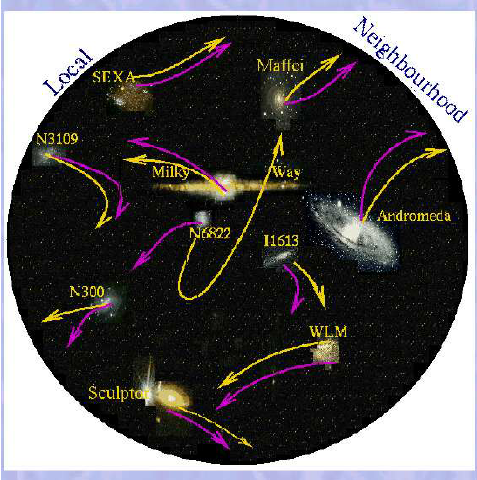
\includegraphics[scale=0.5, angle=0]{peebles.png}
        \caption{Raffigurazione schematica della ricostruzione di Peebles per il Gruppo Locale. Le orbite rosa
        corrispondono alla scelta del minimo dell'azione, mentre quelle gialle indicano la selezione del punto di sella.
        Interessante è il caso della galassia N6822, che offre sia una soluzione in avvicinamento che in allontanamento:
        l'accordo corretto si trova con l'orbita prevista con il punto di sella. Immagine tratta da \cite{mohayaee}.}
		\label{fig:peebles}
	\end{figure}
\end{center}

Tuttavia è impresa ardua ripetere gli stessi risultati su altri set di galassie redshiftate, di cui
sono sconosciute le velocità, necessarie a porre opportune condizioni al contorno. Non è possibile 
quindi scegliere l'orbita corretta tra le molte proposte dall'approccio variazionale, per cui si 
perde l'unicità della soluzione, come accennato in precedenza. 

Oltre all'approccio variazionale appena esposto, un'opzione valida è la ricostruzione POTENT, che si basa
sul rintracciare il campo potenziale della velocità integrando le componenti radiali della velocità.
Questo metodo regge solamente in regime euleriano lineare $|(\rho-\rho_b)/\rho_b|\leq 1$, pertanto non 
recuperano le corrette condizioni iniziali delle regiorni di attuale altà densità, in quanto non lineari:
in altre parole, è un metodo di ricostruzione che non funziona nelle regioni di multistreaming.

Infine il metodo MAK supera sia il problema della non unicità che affligge la ricostruzione di Peebles, 
sia i limiti di validitò dell'algoritmo POTENT, rimanendo valido anche ben oltre il regime lineare euleriano.
Occorre innanzitutto formulare un'equazione di conservazione della massa e prenderla a vincolo

\begin{equation}
    \rho(\bm{x})d\bm{x} = \rho_0(\bm{q})d\bm{q}
\end{equation}
dove $\rho_0(\bm{q})$ è la densità iniziale e a $\rho(\bm{x})$ è la densità alla posizione attuale euleriana.
Manipolando tale equazione di conservazione otterremo 

\begin{equation}
    \label{eqn:masscons}
    \det\left[\frac{\partial q_i}{\partial x_j}\right] = \frac{\rho(\bm{x})}{\rho_0(\bm{q})}
\end{equation}
dove il membro di destra dovrebbe essere noto: conosciamo infatti la posizione della particella
e la densità del campo euleriano, e assumiamo inoltre una densità iniziale costante $\rho_0(\bm{q}) = \rho_0$-
Per risolvere l'equazione, si fa l'ipotesi che la mappa lagrangiana $\mathbb{M}: \bm{q} \mapsto \bm{x}$ si 
possa scrivere come il gradiente di un potenziale convesso $\Phi$.

\begin{equation}
    \bm{x}(\bm{q}, t) = \nabla_q \Phi(\bm{q}, t)
\end{equation}
La convessità del potenziale assicura una relazione biunivoca tra coordinata lagrangiana e coordinata
euleriana, ossia garantisce l'unicità evitando i fenomeni di multistreaming.
Si osserva che nel caso dell'approssimazione di Zel'dovich, con l'equazione (\ref{eqn:zelmap}) che esplicita la 
mappa lagrangiana è possibile costruire il potenziale $\Phi$, che sarebbe dato da 
$\Phi(\bm{q}, t) = \bm{q}^2/2 -a\phi_0(\bm{q}, t)$.
Tuttavia è evidente che tale potenziale non è convesso ovunque, e proprio per questo l'approssimazione
di Zel'dovich non garantisce unicità, in quanto propone una traiettoria rettilinea secondo cui le particelle 
proseguono dritte nella direzione in cui sono entrate nella zona di shell-crossing, in modo abbastanza irrealistico,
dal momento che la traiettoria di una particella che entra in una zona di alta densità viene presumibilmente modificata in modo 
consistente. 
Sarà invece possibile identificare un potenziale convesso e recuperare quindi l'unicità solamente con una proposta 
alternativa all'approssimazione di Zel'dovich, ossia il modello di adesione, che prevede l'aggiunta di 
termini di interazione gravitazionale.
Se $\Phi$ esiste ed è convesso sarà definita convessa anche la mappa inversa $\Theta(\bm{x}, t)$ tale caustiche
$\bm{q} = \nabla_x \Theta$. La relazione tra $\Phi$ e $\Theta$ è stabilita dalle trasformazioni di
Legendre-Fenchel.

\begin{equation}
    \Theta(\bm{x}) = \max_q \{\bm{q}\cdot\bm{x}-\Phi(\bm{q})\} \qquad \Phi(\bm{q}) = \max_x \{\bm{x}\cdot\bm{q}-\Theta(\bm{x})\}
\end{equation}
A questo punto l'equazione (\ref{eqn:masscons}) diventa l'equazione di Monge-Ampere.

\begin{equation}
    \det\left[\frac{\partial^2 \Theta (\bm{x}, t)}{\partial x_i \partial x_j}\right] = \frac{\rho(\bm{x})}{\rho_0}
\end{equation}
Solo recentemente si è scoperto che la soluzione a tale equazione è equivalente alla soluzione unica
di un problema di trasporto ottimo, in particolare il problema di trasporto di massa di Monge-Kantorovich,
in cui si cerca quale relazione tra $\bm{q}$ e $\bm{x}$ minimizza la la funzione quadratica di costo 
$c(\bm{q}, \bm{x}) = |\bm{x}-\bm{q}|^2$, o meglio si cerca la minimizzazione del funzionale I.

\begin{equation}
    \label{eqn:mongeampere}
    I = \int_q \rho_0(\bm{q})|\bm{x}-\bm{q}|^2 d\bm{q} = \int_x \rho(\bm{x})|\bm{x}-\bm{q}|^2 d\bm{x} 
\end{equation}
Si trova infatti che per ottenere la condizione $\delta I = 0$, $\bm{q}(\bm{x})$ deve essere il gradiente
di una funzione di $\bm{x}$. I dettagli della trattazione sono reperibili in \cite{mohayaee} e \cite{matarrese}.
Per risolvere l'equazione (\ref{eqn:mongeampere}) la si discretizza e si risolve il relativo problema di assegnazione 
tramite algoritmi numerici, come quelli presentati in \cite{mohayaee}, che permettano di preservare l'unicità
delle soluzioni.











\begin{comment}
SCALETTA SEGUENTE
nuova sezione con carrellata su metodi di ricostruzione (citare Mohayaee)
- cos'è la reconstruction
- Peebles
- POTENT
- MAK, particolare attenzione perché prende le origini dalla trattazione fluido
ed è il metodo che fornisce unicità
\end{comment}


    \chapter{Tipi di singolarità nella trattazione Lagrangiana}
    
\begin{comment}
    parti fa chiarire con Matarrese

    - non mi torna la definizione di R_tau
    - che significato ha la condizione iniziale xi = -1 + q^3/6...
    - come si posizionano i tempi tau comin e comax rispetto alla linea temporale, o rispetto a tau = 1?
        sono entrambi dopo l'istante tau = 1, perchè sono in shell crossing credo

\end{comment}


\section{Setup e scelta delle condizioni iniziali}

In cosmologia le caustiche, che nascono da una singolarità nella trattazione di fluido esposta nel precedente
capitolo, rappresentano in realtà il processo fondamentale della formazione di strutture a grande scala 
nell'universo. In assenza di questo tipo di singolarità, la materia dell'universo riprodurrebbe in ultimo una
ripartizione omogenea, in coincidenza con il raggiungimento della massima entropia. Tuttavia l'esistenza di queste
divergenze impedisce il conseguimento dell'equilibrio termico, detto in cosmologia \textit{morte termica dell'Universo},
in quanto corrisponderebbe a uno stato ove non sono più possibili scambi di energia. 

Al primo shell-crossing le particelle affrontano invece il \textit{collasso gravitazionale
secondario}, per cui il numero di collisioni aumenta sostanzialmente, e la trattazione si fa delicata. 
ne consegue che la forma oblata del pancake non è l'unica forma che si 
registra: infatti nel contesto di una trattazione nonlineare della dinamica gravitazionale con l'approssimazione
di Zel'dovich si incontrano una serie di strutture scrupolosamente classificate per i casi semplici unidimensionale
e bidimensionale in \cite{arnold}.

Tuttavia la varietà di strutture che può emergere a seguito del collasso gravitazionale non possono essere previste 
da un modello che include l'approssimazione di Zel'dovich, la quale si basa sull'ipotesi di velocità costante.
In effetti si è spiegato nel primo capitolo che ZA risulta essere una soluzione esatta solamente nel caso 
unidimensionale, e in generale valida esclusivamente fino al primo shell-crossing, dove le equazioni del
fluido falliscono. \'E necessario quindi tornare all'equazione di riferimento, ossia all'equazione di Vlasov 
(\ref{eqn:vlasov}), anche limitandosi in prima battuta al caso unidimensionale, dal momento che gli 
shell-crossing si manifestano, almeno nella loro fase iniziale, come fenomeni unidimensionali.


Inquadriamo l'analisi in un universo EdS, dove $\tau = a$ come accennato in precedenza, quando abbiamo anche
fornito la definizione $u(x(q, \tau), \tau) = \partial_a x(q, \tau) = \partial_{\tau}(q, \tau) = \dot{x}(q, \tau)$.
Si riportano le equazioni (\ref{eqn:cont_tau}) e (\ref{eqn:poisson_tau}).

\begin{gather}
    \label{eqn:cont_new}
    \ddot{x} + \frac{3}{2\tau}\dot{x} = - \frac{3}{2\tau}\nabla_x \phi \\
    \label{eqn:poisson_new}
    \laplacian_x\phi = \frac{\delta}{\tau}
\end{gather}
dove si ricorda che $\delta = (\rho - \rho_b)/\rho_b$ rappresenta la deviazione dalla densità media, e sia $\delta$
che $\phi$ dipendono da x. In particolare si può riscrivere 
\begin{equation}
    \label{eqn:density}
    \delta(x(q, \tau), \tau) = \int dq' \delta_D[x(q, \tau)-x(q', \tau)] - 1
\end{equation}
dove $\delta_D$ è una delta di Dirac che dà contributo quando due particelle partite da diverse
posizioni iniziali $q$ e $q'$ collidono nella stessa posizione euleriana $x$.

Si osserva ora che tale set di equazioni gode di invarianza rispetto a trasformazioni di 
Galileo della forma $x \mapsto x + \zeta(\tau)$: possiamo sfruttare questa 
simmetria per imporre una condizione al centro di massa. Per scriverla definiamo il dislocamento
lagrangiano $\xi(q, \tau):= x(q, \tau) - q$.

\begin{equation}
    \label{eqn:com}
    \int_{\mathbb{T}}\xi(q', \tau) dq' = 0
\end{equation}
Se tale condizione non fosse rispettata significherebbe che esiste un certa direzione
privilegiata di moto delle particelle, incompatibilmente con l'ipotesi di assenza di forze esterne.

A questo punto si procede prendendo la divergenza di (\ref{eqn:cont_new}) e inserendovi 
(\ref{eqn:poisson_new}), ottenendo

\begin{equation}
    \nabla_x \ddot{x} + \nabla_x \left(\frac{3}{2\tau}\dot{x}\right) = -\frac{3}{2\tau}\laplacian_x\phi = -\frac{3\delta(x)}{2\tau^2}
\end{equation}
Sostituendo $\nabla_x = \partial_x q \nabla_q$, si ottiene

\begin{gather}
    \nabla_q \ddot{x} + \frac{3}{2\tau} \nabla_q\dot{x} = -\frac{3}{2\tau^2}\frac{\partial x}{\partial q}\delta(x(q,\tau)) \\
    \label{eqn:progress}
    \nabla_q \left[ \tau^2 \partial^2_{\tau} + \frac{3}{2}\tau \partial_{\tau} \right] x = -\frac{3}{2}\frac{\partial x}{\partial q}\delta(x(q,\tau))
\end{gather}
A questo punto definiamo la funzione $F(x(q, \tau))$ come una forza "efficace" di multistreaming, utilizzando 
la definizione della densità (\ref{eqn:density}). Nel dettaglio, $F(x(q, \tau)) = (\partial_q x) \int \delta_D[x(q, \tau)-x(q', \tau)]dq' -1$.
Ma allora il secondo membro della (\ref{eqn:progress}) si può scrivere come

\begin{equation}
    -\frac{3}{2} (\partial_q x )\delta = -\frac{3}{2}(F+1-\partial_q x) = -\frac{3}{2} F +\frac{3}{2} (\partial_q x - 1) = -\frac{3}{2} F + \frac{3}{2} \partial_q \xi    
\end{equation}
dato che in effetti $\partial_q \xi = \partial_q (x-q) = \partial_q x - 1$. 

Il primo membro di (\ref{eqn:progress}) invece contiene un operatore temporale che agisce su $x$. Se si scrive $x(q,\tau) = \xi(q, \tau) + q$ e si nota che q non 
dipende dal tempo, è equivalente far agire l'operatore su $\xi$ anzichè su x. 

\begin{gather}
    \partial_q \left[ \tau^2 \partial^2_{\tau}+\frac{3}{2}\tau\partial_{\tau} \right] \xi = -\frac{3}{2}F(x(q,\tau)) +\frac{3}{2}\partial_q \xi \\
    \label{eqn:Fequation}
    \partial_q \mathcal{R}_{\tau}\xi = -\frac{3}{2}F(x(q, \tau))
\end{gather}
dove si è definito l'operatore $\mathcal{R}_{\tau} = \tau^2\partial^2_{\tau} + (3\tau/2)\partial\tau-3/2$.
Integrando ora la (\ref{eqn:Fequation}) sulla coordinata $q$, sarà possibile ottenere l'equazione 
del moto del dislocamento $\xi$.

\begin{equation}
    \label{eqn:Sequation}
    \mathcal{R}_{\tau}[\xi(q, \tau)-\xi_c(\tau)] = -\frac{3}{2}S(x(q, \tau))
\end{equation}
dove $S$ è definito come l'integrale della forza generalizzata $S = \int_0^q F(q',\tau)dq'$ e $\xi_c$ rappresenta il 
dislocamento alla coordinata $q=0$.
Per potere risolvere l'equazione differenziale espressa nella (\ref{eqn:Sequation}) ci occorrono
però delle condizioni iniziali per l'istante $\tau = 0$.

\begin{equation}
    \label{eqn:initcond}
    \xi(q, 0) = -q + \frac{q^3}{6} + cq^4 + o(q^4) = \xi_{ZA}^{ini}
\end{equation}
in cui si assume c<\!<1. Questa condizione iniziale viene dall'applicare
un'espansione di Taylor al potenziale gravitazionale, sapendo che quest'ultimo, nell'approssimazione di Zel'dovich, 
esatta in una dimensione, è collegato alla velocità, come evidente in (\ref{eqn:zelsol}), dove si osserva che la 
velocità non è altro che la derivata del potenziale (\cite{zeldovich}). Proviamo dunque a espandere il potenziale

\begin{gather}
    \label{eqn:phiexp}
    \phi(q) = \phi_0 + a_1 q + a_2 q^2 + a_3 q^3 + a_4 q^4 + a_5 q^5 + O(q^6) \\
    \phi'(q) = a_1 + 2 a_2 q + 3 a_3 q^2 + 4a_4q^3 + 5a_5 q^4 + O(q^5) \\
    \phi''(q) = 2a_2 +6a_3 q + 12a_4 q^2 + 20a_5 q^3 + O(q^4) \\
    \phi'''(q) = 6a_3 + 24 a_4 q + 60a_5 q^2 + O(q^3) 
\end{gather}
dove $a_i = (1/i!) \phi^{(i)}(0)$.
La derivata seconda del potenziale è tuttavia esprimibile tramite gli autovalori $\lambda(q)$ del tensore di deformazione,
come mostrato nel capitolo precedente. Pertanto, nel momento in cui si adotta l'ipotesi di massimo per tale autovalore, cioè
si ricerca il primo istante di shell-crossing, poniamo la derivata seconda del potenziale nulla. Si chiede dunque $\lambda'(q)=0$, 
cioè $\phi'''(0)=0$. Pertanto è automatica la
scelta $a_3 = 0$, che priva la derivata prima $\phi'(q)$, e con essa la velocità, della potenza quadratica.
L'espansione proposta in (\ref{eqn:phiexp}) è quella proposta in \cite{rampf} e permette di disporre del termine di quarto grado 
nella velocità, come espresso in (\ref{eqn:initcond}), mentre in \cite{colombi} ci si ferma a gradi inferiori.

Finchè non vi sono eventi di collisione, ossia nella regione di single-stream, non si verificano 
sovrapposizioni tra coordinate euleriane generate da diversi antecedenti lagrangiani, ossia $x(q)\neq x'(q')$.
Questo rende l'espressione di densità (\ref{eqn:density}) nulla, e con essa anche la forza generalizzata
$F(x(q, \tau)$ e il suo integrale $S(x(q, \tau)$. Pertanto  in regime di single-stream l'equazione (\ref{eqn:Sequation}) si riduce
a $\mathcal{R}_{\tau}[\xi(q, \tau)-\xi_c(\tau)] = 0$. Sfruttando inoltre la condizione del centro di 
massa (\ref{eqn:com}), imponiamo $\xi_c = 0$, recuperando così la soluzione di Zel'dovich.

\begin{equation}
    x_{ZA}(q, \tau) = q+ \tau \xi_{ZA}^{ini}
\end{equation}
Sappiamo che tale soluzione risulta valida solamente fino al primo shell-crossing, momento in cui si verifica
la condizione $\partial_q x_{ZA} = 0$, che causa invece la divergenza della densità prima nulla.
Infatti, ricordando la proprietà della delta di Dirac

\begin{equation}
    \label{eqn:dirac}
    \delta_D(f(x)) = \sum_i \frac{\delta_D(x-a_i)}{f'(a_i)}
\end{equation}
dove $\{a_i\}$ sono gli zeri di $f(x)$, si trova che la (\ref{eqn:density}) diventa

\begin{equation}
    \label{eqn:density_ZA}
    \delta(x_{ZA})= \int dq' \delta_D[x(q, \tau) - x(q', \tau)] - 1 = \int dq' \frac{\delta_D(q' - q)}{\partial_q x_{ZA}(q, \tau)} - 1 = \frac{1}{\partial_q x_{ZA}}-1
\end{equation}
per cui si è chiarito perché la densità diventa infinita quando $\partial_q x_{ZA} = 0$.

Inoltre, grazie alla scelta delle condizioni iniziali, il primo shell crossing è posto a $\bar{\tau}=1$.


\section{Evoluzione post-Zel'dovich}

Dopo lo shell-crossing è necessario rinunciare alla soluzione analitica della (\ref{eqn:Sequation}) per 
fare uso invece di un algoritmo iterativo, il cui primo ciclo adotterà come forza generalizzata la
$F(x_{ZA}(q, \tau))$ calcolata sull'ultima $x_{ZA}$ ricavata dall'approssimazione di Zel'dovich.

\begin{equation}
    \mathcal{R}_{\tau}[\xi_{PZA}(q, \tau)-\xi_c(\tau)] = -\frac{3}{2}S_{ZA}(q, \tau)
\end{equation}
Per determinare $S_{ZA}(q, \tau)$ occorre cercare le condizioni per cui si cancella l'argomento 
della delta di Dirac con cui è costruita la forza generalizzata. Svolgendo i calcoli, si trova
che l'argomento della delta di Dirac si annulla per tre radici $q_1$, $q_2$ e $q_3$, per cui, 
utilizzando la proprietà (\ref{eqn:dirac}), è possibile riscrivere $F(x_{ZA}(q, \tau))$ come

\begin{equation}
    F(x_{ZA}(q, \tau)) = \partial_q x_{ZA}(q)\left[\frac{1}{\partial_q x(q_1)} + \frac{1}{\partial_q x(q_2)} + \frac{1}{\partial_q x(q_3)}\right]
\end{equation}
A questo punto ci è possibile calcolare $S_{ZA}$: attraverso la teoria delle perturbazioni si ricava,
per coefficienti $c$ piccoli, il seguente risultato.

\begin{equation}
    \label{eqn:SZA}
    S_{ZA} = 
    \begin{cases}
        0 & 0 \leq \tau \leq \tau_{com} \\
        -sign(q)\sqrt{D(q, \tau, c)} & \tau_{com} \leq \tau \leq \tau_{min} \\
        -3q & \tau_{min} \leq \tau
    \end{cases}
\end{equation}

dove $D(q, \tau, c) = 24 - 3q^2 -42/\tau + 24cq(3-1^2-3/\tau)$, mentre i due tempi che separano 
i tre diversi andamenti sono dati da $\tau_{com} = 8/(8-q^2-5cq^3)$ e $\tau_{min} = 2/(2-q^2-8cq^3)$.
Tramite questi tempi sono definite le coordinate lagrangiane $q_{max}$ e $q_{comax}$, che sono le 
coordinate lagrangiane associate alla posizione euleriana massima $x_{max}$ che delimita l'estremo
superiore della zona di multistreaming, e $q_{min}$ e $q_{comin}$, associate all'altro estremo 
della zona di multistreaming $x_{min}$. 

$S_{ZA}$ ci è necessaria per il primo ciclo del calcolo iterativo di $\xi_{PZA}$, ma occorre anche
conoscere il valore della costante di integrazione $\xi_c(\tau)$. Per determinarla definiamo 
$M(q, \tau) = \mathcal{R}_{\tau} \xi_c (\tau)- 3/2 S_{ZA}(q,\tau)$, da cui possiamo scrivere, 
riordinando la (\ref{eqn:Sequation}) e integrando per $q \in [-\pi, \pi]$, la seguente.

\begin{equation}
    \int_{-\pi}^{\pi} \mathcal{R}_{\tau}\xi_{PZA}(q', \tau)dq' = \int_{-\pi}^{\pi} M(q', \tau) dq'
\end{equation}
In tale equazione si può far uso della condizione (\ref{eqn:com}) per cancellare il membro di sinistra
e ottenere quindi che l'integrale di $M$ deve essere nullo. Questo integrale risulta problematico
per via della definiziona tratti di $S_{ZA}$ (\ref{eqn:SZA}), per cui facciamo l'ipotesi forte 
$\xi_c = \xi_1 + \xi_2 + \xi_3$ dove le $\{\xi_i\}$ sono soluzioni individuali delle tre regioni 
di definizione, cioè le costanti di integrazione di ciascun tratto.

Imporre $\int_{-\pi}^{\pi} M(q', \tau) dq' = 0$ equivale a chiedere 
$\int_{-\pi}^{\pi} \mathcal{R}_{\tau}\xi_c(q', \tau) dq' = \int_{-\pi}^{\pi} \frac{3}{2} S_{ZA}(q', \tau) dq'$
ma dato che $\xi_c$ è indipendente da $q$ la stessa equazione si può riscrivere come

\begin{equation}
    \mathcal{R}_{\tau} \xi_c(\tau) = \Big\langle \frac{3}{2}S_{ZA}(q, \tau) \Big\rangle
\end{equation}
Questa stessa equazione, ripartita nei vari regimi, si traduce nel seguente gruppo di equazioni

\begin{gather}
    \label{eqn:xi1}
    \mathcal{R}_{\tau} \xi_1(\tau) = 0 \\
    \label{eqn:xi2}
    \mathcal{R}_{\tau} \xi_2(\tau) = - \Big\langle \frac{3}{2} sign(q) \sqrt(D(q, \tau, c)) \Big\rangle = 18c (1-\frac{1}{\tau}) \\
    \label{eqn:xi3}
    \mathcal{R}_{\tau} \xi_3(\tau) = - \Big \langle \frac{9}{2} q \Big \rangle = 36c (1-\frac{1}{\tau})\Big\rangle 
\end{gather}
La soluzione della (\ref{eqn:xi1}), nel regime di single stream, è data da $\xi_1=0$, mentre (\ref{eqn:xi2}) 
e (\ref{eqn:xi3}) richiedono l'utilizzo delle condizioni iniziali $\xi(\tau=1)=0$ e $\dot{\xi}(\tau=1)=0$.
Si ottengono dunque delle soluzioni valide per $\xi_i$, che sommate danno luogo al valore della costante
di integrazione $\xi_c$.

\begin{equation}
    \label{eqn:xic}
    \xi_c(\tau)= -\frac{18c}{5}\left(10+8\tau^{-\frac{2}{3}}-\frac{15}{\tau}-3\tau\right)
\end{equation}
Si osserva che $\xi_c$, che si attiva solamente dopo il primo shell crossing, ossia a $\tau=1$,
ossia è interpretato come un boost dipendente dal tempo che non sarebbe prevedibile con l'appoggio
della sola approssimazione di Zel'dovich.

In (\ref{fig:fig1}) è rappresentato il moto della particelle nell'istante $\tau=1.002$, ovvero
poco dopo il primo shell-crossing.

\begin{center}
    \begin{figure}[H]
        \centering
        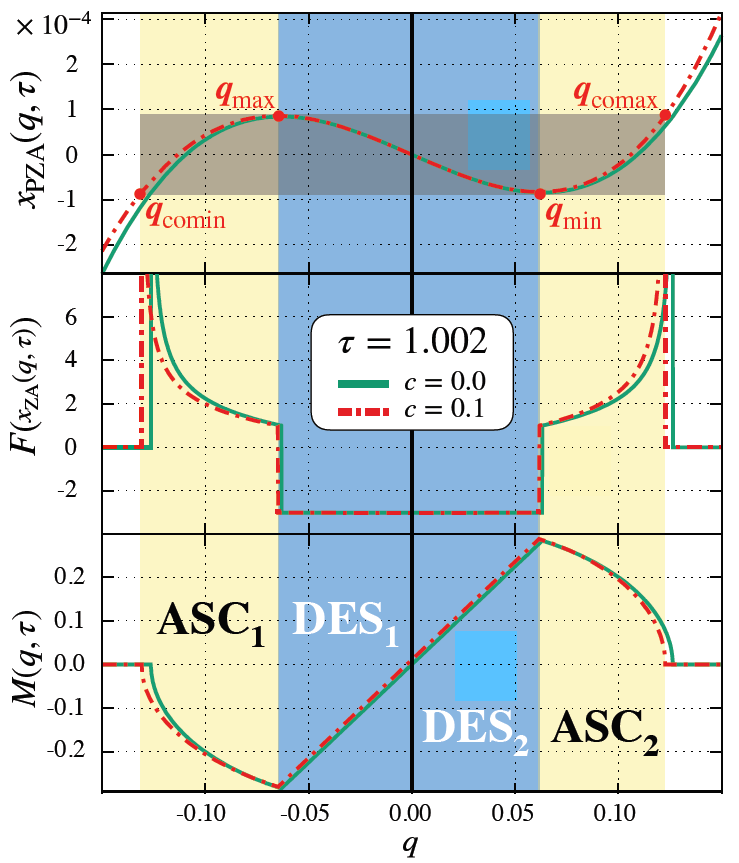
\includegraphics[scale=0.5, angle=0]{fig1.png}
        \caption{Nel pannello in alto è raffigurata un'immagine della mappa post-Zeldovich a $\tau=1.002$,
        nel pannelo centrale e quello inferiore sono mappate rispettivamente $M(q, \tau)$ e $F(q, \tau)$.
        La linea verde rappresenta la soluzione con c = 0, mentre la linea rossa tratteggiata è la soluzione
        con c = 0.1. Nel pannello in alto la zona grigia corrisponde alla zona di multistreaming, dove si
        vede che a una stessa posizione x possono corrispondere più posizioni iniziali $q$. Inoltre il primo 
        pannello definisce due regioni verticali \textit{ascending} e \textit{descending}.
        Si osserva inoltre, nel secondo pannello, la presenza di punti con derivata discontinua della forza
        generalizzata, corrispondenti a effetti di singolarità fisiche. Figura tratta da \cite{rampf}
        }
        \label{fig:fig1}
	\end{figure}
\end{center}

Ricavata dunque una soluzione per $\xi_c$ è possibile tornare all'equazione (\ref{eqn:Sequation}) 
e risolvere per $\xi_{PZA}$ utilizzando il metodo di variazione delle costanti su 
$\xi_{PZA} = \lambda(\tau)\tau + \mu(\tau)\tau^{-3/2}$ adottando le condizioni iniziali 
$\xi_{PZA}(\tau = 1) = \xi_{ZA}^{ini}$ e $\dot{\xi}_{PZA}=\xi_{ZA}^{ini}$. Su queste basi si 
ricava

\begin{equation}
    \label{eqn:finale}
    \xi_{PZA} = \xi_c(\tau) + 
    \begin{cases}
        \tau \xi_{ZA}^{ini}(q) & 0 \leq \tau \leq \tau_{com} \\
        \tau \xi_{ZA}^{ini}(q) +\frac{sign(q)}{180} \frac{D^{\frac{5}{2}}(q, \tau, c)\tau}{8-q^2+cq(48-11q^2)} & \tau_{com} \leq \tau \leq \tau_{min} \\
        -3q + \frac{4}{5}q\tau -\frac{17}{60}q^3\tau +\frac{48}{5} \sqrt{\frac{2}{2-q^2}} \frac{q}{8-q^2}\tau^{-\frac{3}{2}}+cf(q, \tau) & \tau_{min} \leq \tau
    \end{cases}
\end{equation}
d0ve la definizione di $D(q, \tau, c)$ è stata fornita in precedenza, mentre 


\begin{equation}
    f(q, \tau) = \frac{11}{20}q^4\tau -\frac{36}{5}q^4\left(\frac{2}{2-q^2}\right)^{3/2}\frac{3q^2-4}{(q^2-8)^2}\tau^{-\frac{3}{2}}.
\end{equation}

La (\ref{eqn:finale}) fornisce quindi l'andamento complessivo del dislocamento $\xi$. In figura (\ref{fig:fig2}) è proposto un confronto
tra previsione teorica e simulazione a N corpi.


\begin{center}
    \begin{figure}[H]
		\centering
		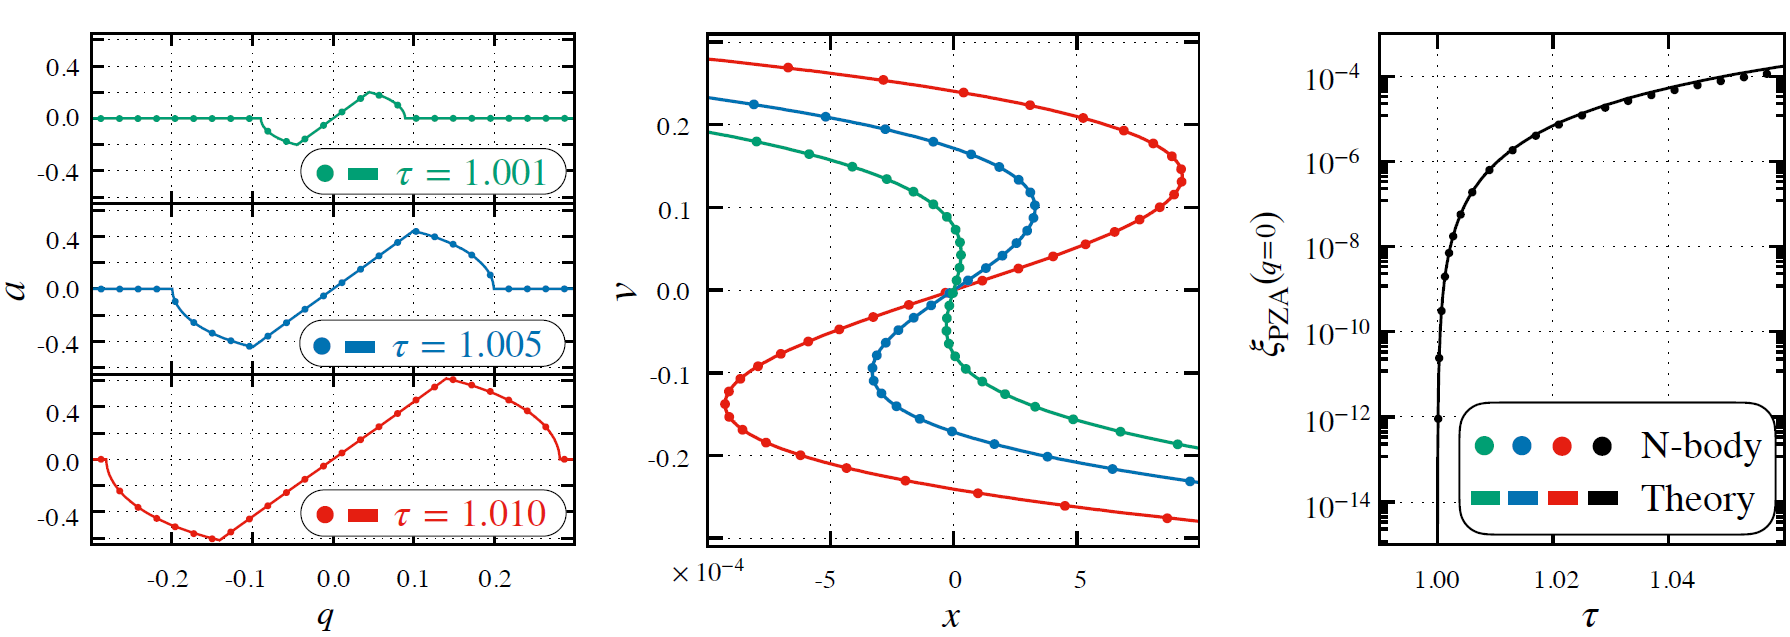
\includegraphics[scale=0.35, angle=0]{fig2.png}
        \caption{Confronto tra predizione teorica (linea continua) e simulazione a N corpi (punti).
        Il pannello di sinistra raffigura l'accelerazione $\ddot{\xi_{PZA}}$ per $c$=0, in cui è possibile 
        visualizzare alcuni punti a derivata discontinua che rivelano le singolarità fisiche, ben riprodotte 
        anche dall'andamento della simulazione. Il pannello centrale raffigura le orbite nello spazio delle fasi 
        $(x, v)$ sempre con $c$=0. Il pannello di destra invece raffigura l'improvviso valore non nullo di $\xi_{PZA}$
        al primo shell-crossing ($\tau = 1$), in conseguenza dell'attivazione della forza di multistreaming all'istante
        $\tau = 1$, costruita con $c$=0.1. Figura tratta da \cite{rampf}.
        }
        \label{fig:fig2}
	\end{figure}
\end{center}

\section{Singolarità nello spazio e nel tempo}
\label{sec:sing}

Nel precedente capitolo si è ottenuta infine l'equazione del dislocamento $\xi_{PZA}(q,\tau)$, definita in tre
diverse regioni temporali. Tale equazione (\ref{eqn:finale}) presenta delle singolarità che è possibile classificare
principalmente in due gruppi: singolarità di tipo (a), cioè quelle definite all'interno della regione temporale, e 
singolarità di tipo (b), che invece emergono quando si cerca di imporre la continuità di $\xi_{PZA}$ attraverso
le regioni di definizione. 

Una singolarità di tipo (a) si riscontra all'annullarsi della funzione $D(q, \tau, c)$, fatto che si verifica quando 
$\tau = \tau_{com}$ e se si sceglie al contempo c=0. Per investigare tal singolarità diventa necessario sviluppare
in espansione di Taylor la funzione $D$ per piccole deviazioni $\delta\tau>0$ intorno a $\tau_{com}$. Da tale espansione
si troverà che il termine dominante per $\xi_{PZA}$è del tipo $\delta\tau^{5/2}$. Un ragionamento del tutto analogo si presenta 
se l'espansione invece si compie su $q$ fissando l'istante $\tau$ ed espandendo dunque intorno a $q_{comax}$ o $q_{comin}$:
in tal caso si presenterà un termine dominante $q^{5/2}$. 

Troviamo anche due singolarità di tipo (b): la prima si verifica all'istante $\tau_{min}$, cioè quando si incollano 
le due regioni a cavallo di tale istante, che sono rispettivamente ascending e descending. Per poter realizzare la 
condizione di continuità, è sufficiente, come prima, porre $c$=0. Di nuovo espandendo con Taylor intorno a  $\tau = 
\tau_{min}$ si trova che la derivata terza di $\xi_{PZA}$ cambia segno presso tale punto. Pertanto in un intorno 
di $\tau_{min}$ il dislocamento deve assomigliare a una funzione $(\tau-\tau_{min})^3 \theta(\tau-\tau_{min})$.
Anche la derivata terza spaziale risulta essere discontinua
Sia la prima singolarità di tipo (a) che quella di tipo (b) sono rappresentate nel pannello di sinistra della figura
(\ref{fig:fig2}), che riporta una soluzione con $c$=0.

Infine è presenta anche una terza singolarità, sempre di tipo (b), che viene dalla definizione di $\xi_c$ in (\ref{eqn:xic}):
infatti si è osservato in precedenza che $\xi_c$ funge da boost che si attiva al primo shell-crossing entrando nella 
regione di multistreaming, passando quindi da zero a un valore improvvisamente non nullo. Per questo motivo la particella,
che inizialmente procede con velocità costante, acquista bruscamente un'accelerazione non nulla, secondo un andamento
non olomorfo (analitico). Questa tipo di singolarità si può osservare nel terzo pannello di (\ref{fig:fig2}), dove è
raffigurato l'andamento di $\xi_{PZA}$ con $c$=0.1.

Sempre in (\ref{fig:fig2}) è effettuata una comparazione tra i risultati analitici (linea continua) e una simulazione 
a N corpi della dinamica (punti): il codice usato per la simulazione tratta il caso unidimensionale, è simplettico
e si basa su un algoritmo che determina la forza di multistreaming, partendo da condizioni iniziali stabiliti con
l'approssimazione di Zel'dovich, che governa il regime a single-stream, e tramite l'equazione (\ref{eqn:com}).
Si può osservare che l'accordo tra previsione teorica e dati simulativi è eccellente.


    \chapter*{Conclusioni}
    La definizione di $\xi_{PZA}$ in regioni di validità ha permesso di guidare una ben precisa
categorizzazione delle singolarità, come esposto nella sezione \ref{sec:sing}: si è 
parlato di due tipi diversi di singolarità che possiamo definite locali, uno interno alle 
regioni di definizione, uno derivato dal tentativo di imporre le condizioni di continuità 
tra due regioni consecutive.
Vi è tuttavia un terzo tipo di singolarità, di tipo globale, ed è legato alla scelta della
costante di integrazione $\xi_c(\tau)$ in (\ref{eqn:Fequation}).

\begin{comment}
    qui non ben chiaro cosa si intende per spatial average
\end{comment}

La determinazione di $\xi_c(\tau)$ è di fondamentale importanza in quanto tale costante 
di integrazione rappresenta il boost galileiano che agisce sulle posizioni di tutte le 
particelle nella fase \textit{descending} del regime di multistreaming.

E' importante ribadire che la trattazione esposta in questo elaborato e in \cite{rampf}
è tutta nel caso unidimensionale: ad ogni modo, le equazioni di base (\ref{eqn:cont_new}),
(\ref{eqn:poisson_new}), (\ref{eqn:density}) e (\ref{eqn:com}) sono facilmente estendibili
anche al caso tridimensionale. Sarà inoltre necessario utilizzare LPT a ordini superiori,
con l'accortezza di scegliere opportune condizioni al contorno per lo shell-crossing.
Una teoria pienamente sviluppata, basata quindi sull'equazione di Vlasov Poisson 
(\ref{eqn:vlasov}), darebbe accesso ad avanzate predizioni teoriche. In particolre è possibile
fornire i cosiddetti \textit{theoretical inputs} per la scrittura di teorie efficaci di uso 
frequente, spalleggiate da simulazioni a N corpi.

L'equazione di Vlasov-Poisson offre varie applicazioni aldilà dell'utilizzo in 
cosmologia: difatti ha un ruolo chiave in fisica dei plasmi.

    \printbibliography
    
\end{document}